\chapter{\Zee\ cross section measurement}
\label{sec:ZeeCrossSec}

The measurement of the \Zee\ production cross-section is the main purpose of this work, and the details of the methodology of the measurement are discussed in this chapter.

The ATLAS detector, like every other physical device, has its limitations, and the signal obtained from the detector is thus distorted. The process of estimating the results that would have been achieved with an ideal detector based on the results using the real detector is called the unfolding process (also called "deconvolution" or "unsmearing" in mathematical literature), and is the one of the most important stages of the measurement of the cross-section. The main idea of the unfolding is that if $f_\mathrm{meas}(x)$ is the spectrum of a value measured using the real detector and $f_\mathrm{truth}(x)$ is the the spectrum that would have been measured with an ideal detector, then
\begin{equation}
f_\mathrm{meas}(x) = \int R(x|y) \, f_\mathrm{truth}(y)dy
\end{equation}
where $R(x|y)$ is the detector response function. In case of binned distribution this equation can be written as
\begin{equation}
v^\mathrm{meas}_i = \sum_j R_{ij} \, v^\mathrm{truth}_j \:\:\:\:\: i,j = 1, ... ,N
\end{equation}
where $v^\mathrm{meas}_i$ and $v^\mathrm{truth}_i$ are the measured and ideal values accordingly. Generally speaking, the number of bins in $v^\mathrm{meas}$ and $v^\mathrm{truth}$ spectra can be different, and the matrix $R_{ij}$ would be rectangular, but in this analysis the same binning is used for both. The main task of unfolding is to determine the response matrix, and then to calculate the unfolding matrix based on it. The easiest solution would be to just invert the response matrix:
\begin{equation}
v^\mathrm{truth}_i = \sum_j R^{-1}_{ij} \, v^\mathrm{meas}_j \:\:\:\:\: i,j = 1, ... ,N
\end{equation}
which is not always the best choice, because it produces very large distortions in case of limited statistics. The task of propagating the systematic uncertainties through the unfolding process also must be solved.

There are two methods of unfolding that are usually employed by ATLAS analysis groups: the bin-by-bin correction, and the Bayesian unfolding~\cite{lib:zcs_unfolding}. There are several advantages and disadvantages in both methods, but the main criteria of the preference of the Bayesian or bin-by-bin unfolding lies in two important factors: purity and stability. These two factors are calculated as follows:
\begin{equation}
P^{i} = \frac{N^{i}_{\text{rec\&gen}} }{ N^{i}_{\text{rec}} }\,, \; \;
S^{i} = \frac{N^{i}_{\text{rec\&gen}} }{ N^{i}_{\text{gen}} }\,,
\end{equation}
where:
\begin{itemize}
\item {\bfseries $N^i_{\text{rec\&gen}}$} is the sum of event weights which were generated and reconstructed in bin $i$.
\item {\bfseries $N^i_{\text{rec}}$} is the sum of event weights reconstructed in bin $i$.
\item {\bfseries $N^i_{\text{gen}}$} is the sum of event weights generated in bin $i$.
\end{itemize}

The purity is thus a measure of in-migration, which shows the amount of foreign events reconstructed in the given bin, while the stability is a measure of the out-migration, which shows the amount of events that were reconstructed in other bins for every given bin. In terms of response matrix, the distribution with high purity and stability will have a mostly diagonal matrix. This will warrant for a use of a bin-by-bin unfolding. This method, dealing with every bin independently, will produce a diagonal matrix. But if the migrations between bins are substantial, ignoring it will highly increase the distortions in the unfolded results, in which case the Bayesian unfolding becomes preferable. The results of the purity and stability studies for the \Zee\ central-forward analysis suggested that the Bayesian unfolding would be more effective (see Figure~\ref{fig:ZeeCS_purity_stability} for the exact values of the purity and stability of the 2011 \Zee\ central-forward analyses). In the following sections the methodology for both bin-by-bin and Bayesian unfoldings are shown. Also, the methodology of the result combination is explained, which mathematically is very close to unfolding, as it is the same inverse problem (when the same distribution is measured with several partially independent methods, their combination becomes a complicated task).

\begin{figure}
  \centering
  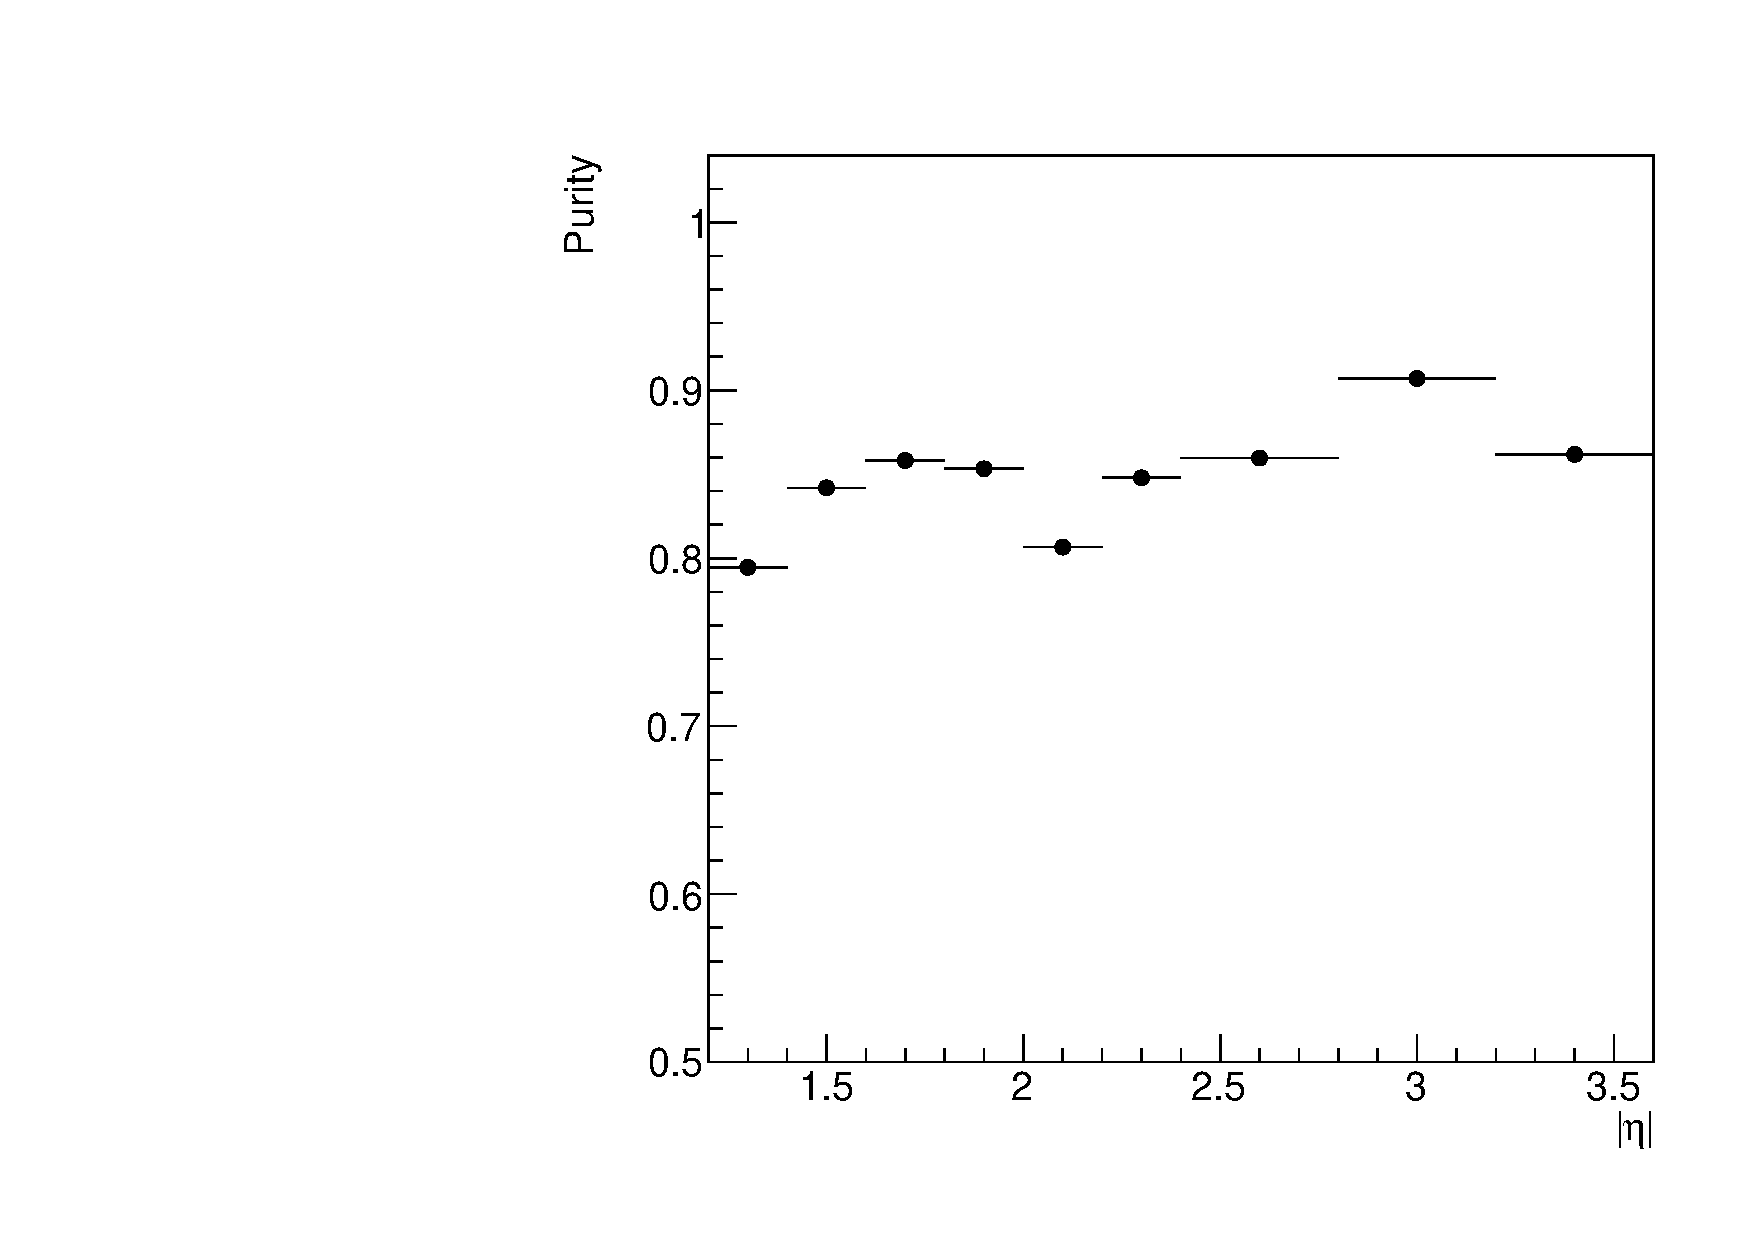
\includegraphics[width=0.45\textwidth]{figures/ZCF_purity_peak}
  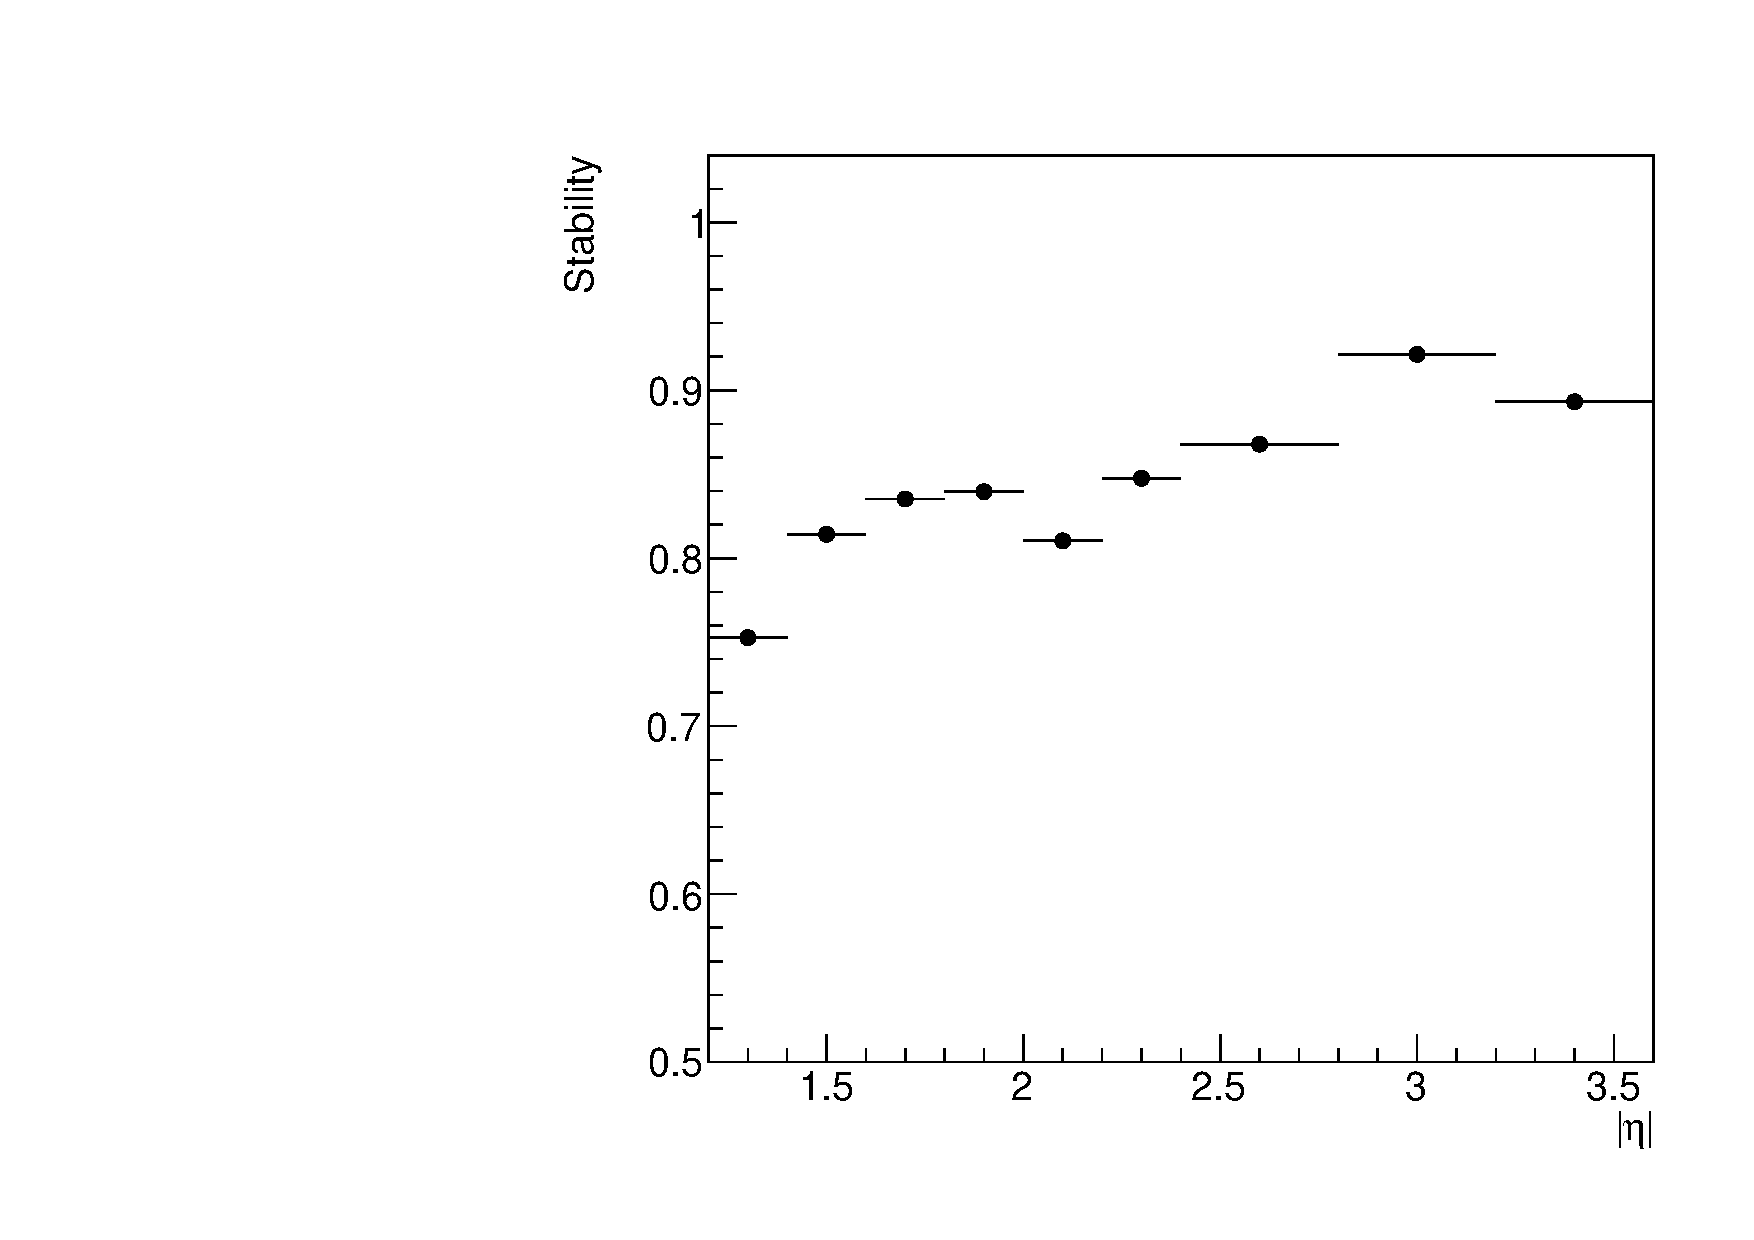
\includegraphics[width=0.45\textwidth]{figures/ZCF_stability_peak} \\
  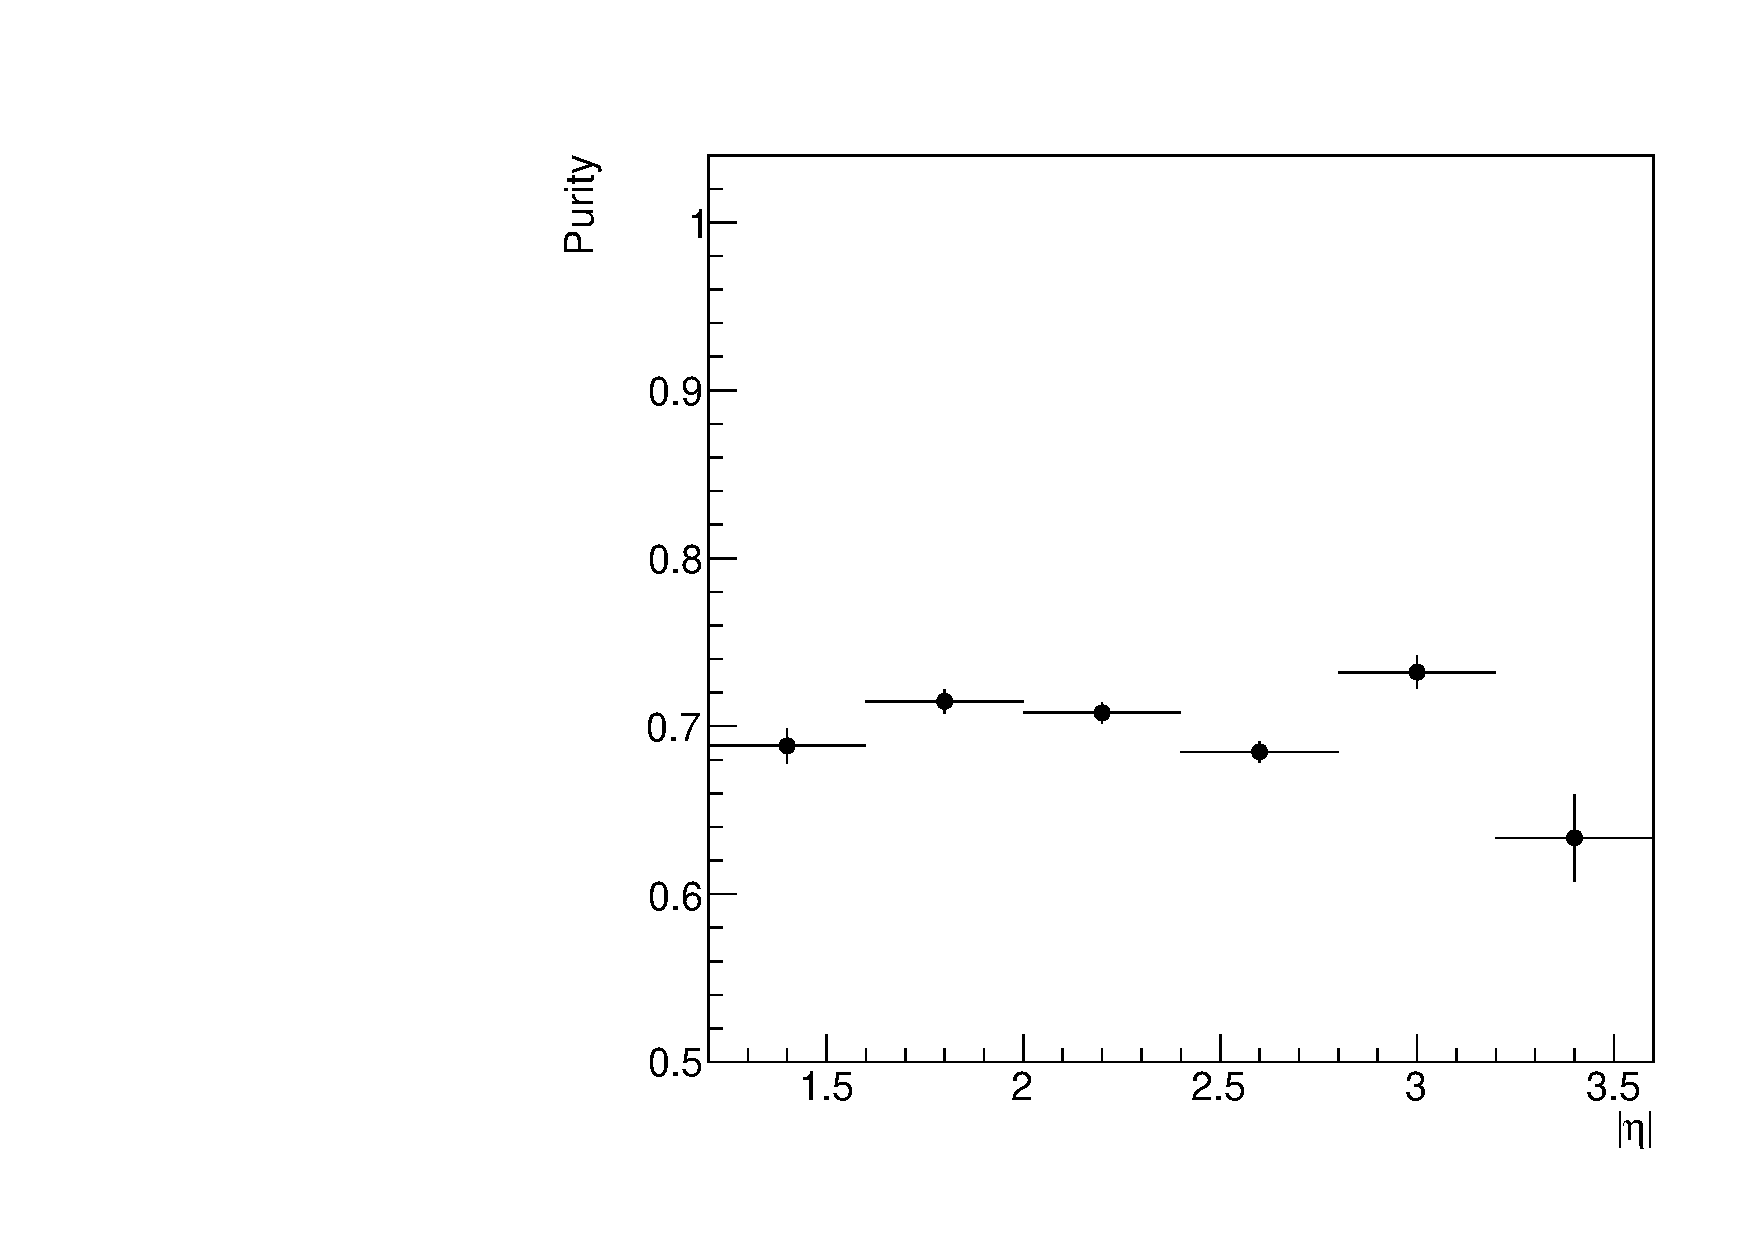
\includegraphics[width=0.45\textwidth]{figures/ZCF_purity_high}
  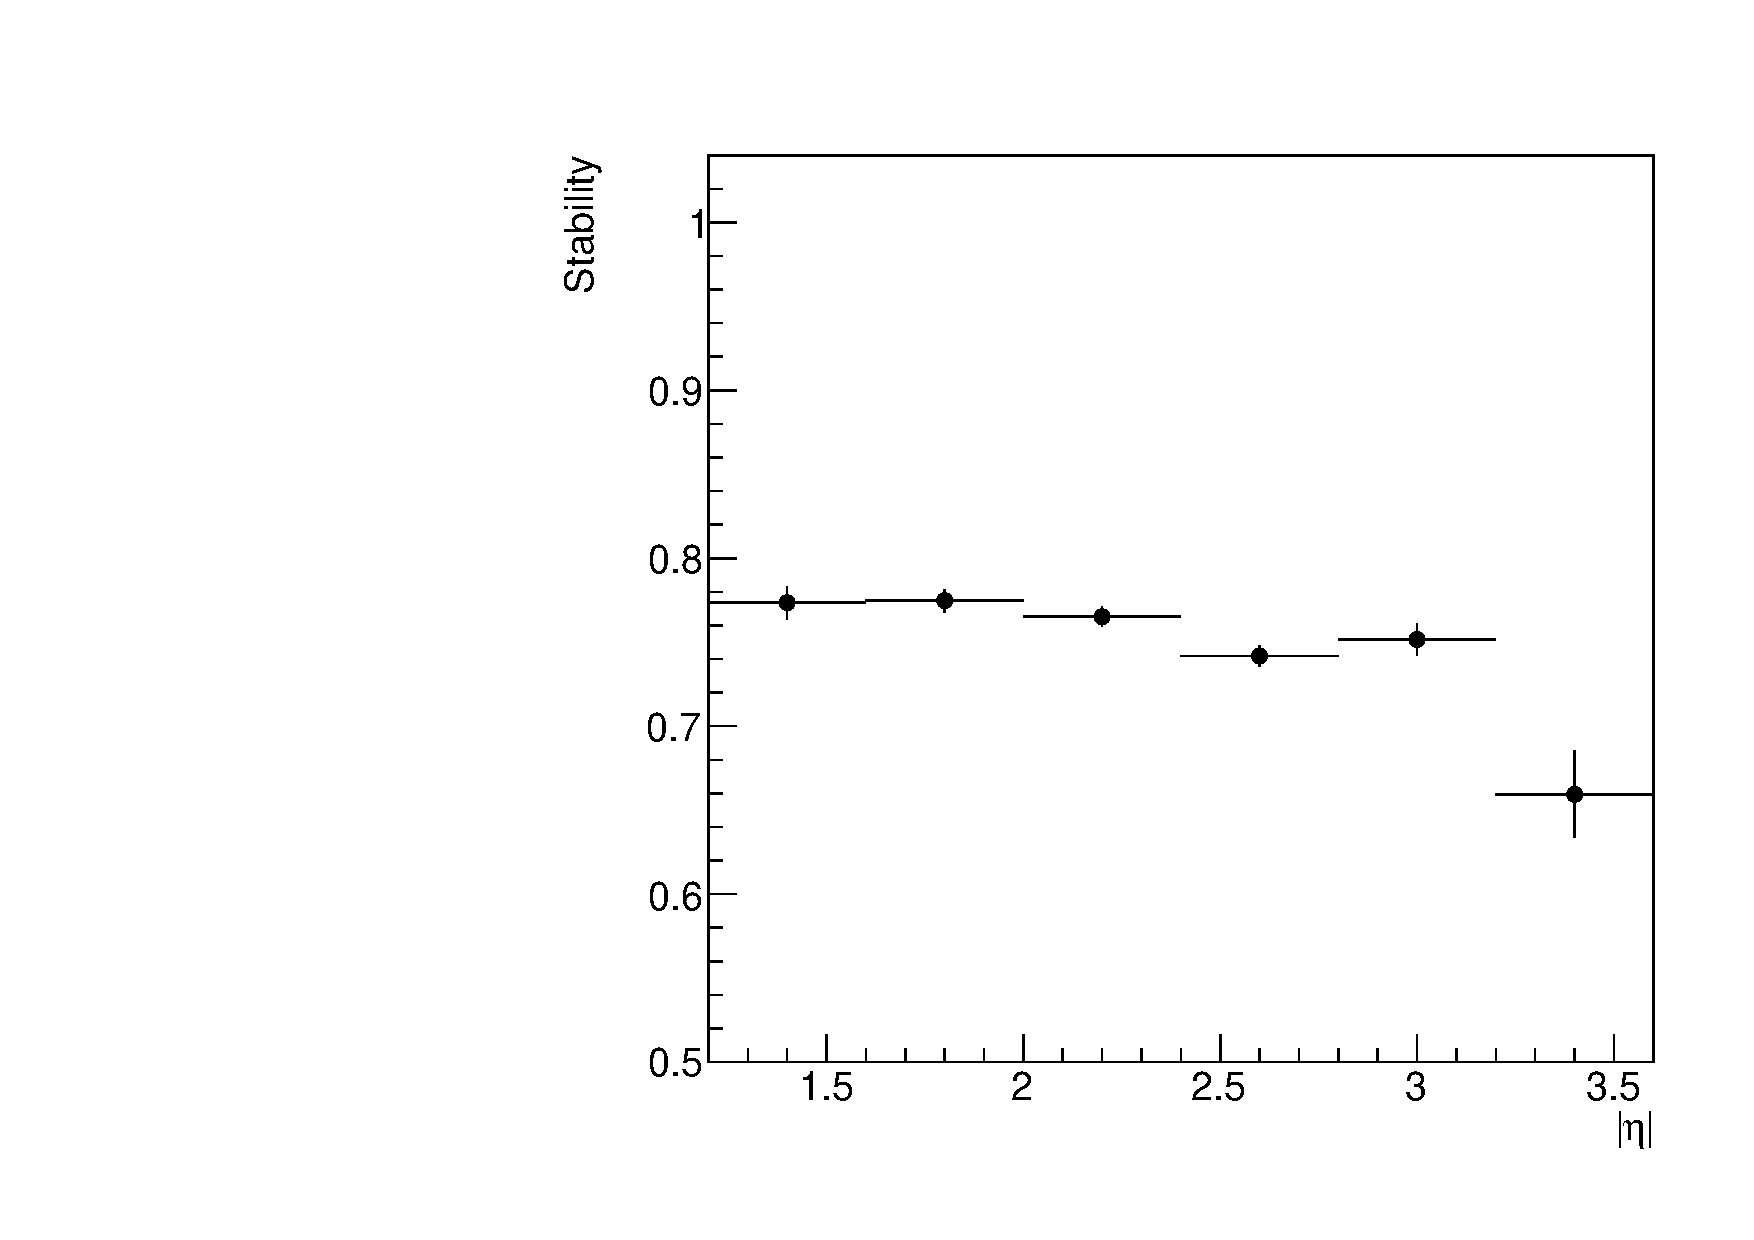
\includegraphics[width=0.45\textwidth]{figures/ZCF_stability_high} \\
  \caption{Purity (left) and stability (right) for the Z central-forward peak mass (top) and high mass (bottom) analyses. The plots were made using the \Zee\ MC samples with standard CF analysis cuts.}
  \label{fig:ZeeCS_purity_stability}
\end{figure}

The differential cross-section measurement was done in absolute rapidity binning.
The binning is the same for CC and CF analyses in the region that is covered with both of them, which allows for the easy combination of the results. The binning is shown in Tabs.~\ref{tab:ZeeCS_bins_peak} and~\ref{tab:ZeeCS_bins_high}. The mass binning for the double-differential CF analysis had only two bins: the peak-mass window $66 < m_{ee} < 116$~GeV and the high-mass window $116 < m_{ee} < 150$~GeV.

\begin{table}
\centering
\begin{tabular}{c}
\hline\hline
Boundaries\\\hline
$1.20 < |y_{Z}| <1.40$\\
$1.40 < |y_{Z}| <1.60$\\
$1.60 < |y_{Z}| <1.80$\\
$1.80 < |y_{Z}| <2.00$\\
$2.00 < |y_{Z}| <2.20$\\
$2.20 < |y_{Z}| <2.40$\\
$2.40 < |y_{Z}| <2.80$\\
$2.80 < |y_{Z}| <3.20$\\
$3.20 < |y_{Z}| <3.60$\\
\hline\hline
\end{tabular}
\caption{Bins in $|y_{Z}|$ which are used for the \Zee\ CF analysis for peak mass window ($66 < m_{ee} < 116$~GeV).}
\label{tab:ZeeCS_bins_peak}
\end{table}

\begin{table}
\centering
\begin{tabular}{c}
\hline\hline
Boundaries\\\hline
$1.20 < |y_{Z}| <1.60$\\
$1.60 < |y_{Z}| <2.00$\\
$2.00 < |y_{Z}| <2.40$\\
$2.40 < |y_{Z}| <2.80$\\
$2.80 < |y_{Z}| <3.20$\\
$3.20 < |y_{Z}| <3.60$\\
\hline\hline
\end{tabular}
\caption{Bins in $|y_{Z}|$ which are used for the \Zee\ CF analysis for high mass window ($116 < m_{ee} < 150$~GeV).}
\label{tab:ZeeCS_bins_high}
\end{table}

\section{Bin-by-bin unfolding}
\label{sec:ZCS_bbb_unf}

The bin-by-bin unfolding doesn't take into account the migrations between bins, and works with every bin separately. The unfolded value can be translated into the cross-section value, and the formulae for both integrated and differential cross-sections are:
\begin{equation}
\sigma_{tot} = \sigma_{Z} \times BR(\Zee) = \frac{N - B}{C \cdot E \cdot A \cdot L_{int}  \cdot \Gamma}\,,
\end{equation}
where:
\begin{itemize}
\item {\bfseries $N$} is the number of candidate events measured in data.
\item {\bfseries $B$} is the number of background events (see Section~\ref{sec:Bkg} for further information on the background estimation).
\item {\bfseries $L_{int}$} is the integrated luminosity corresponding to the dataset.
\item {\bfseries $\Gamma$} is the bin width for differential measurements. Measurements in rapidity quantities $\eta$ and $y$ are done in absolute binning as final value, therefore $\Gamma$ for them is doubled.
\item $C$, $E$, and $A$ are efficiency-acceptance corrections calculated from (binned) sum of weights of MC events generated or reconstructed with analysis cuts applied. They take the uncorrected event yield in steps to different levels:
\begin{itemize}
\item The coefficient for a \textit{genuinely experimental fiducial volume in each channel} as defined by the individual cuts is reached after dividing by
\begin{equation}
  C = \frac{N_\mathrm{MC, rec}}{N_\mathrm{MC, gen, cutexp}}\,.
\end{equation}
$C$ is corrected for any discrepancy in the electron efficiencies between data and MC as described in Section~\ref{sec:Efficiency}. Here the sum of weights of MC events generated after experimental fiducial acceptance cuts ($N_\mathrm{MC, gen, cutexp}$) and the sum of weights of MC events after simulation, reconstruction and experimental selection ($N_\mathrm{MC, rec}$) enter.
\item The coefficient for a \textit{common fiducial volume} is a theoretical extrapolation designed to unify the fiducial volumes of different flavors of \Zll\ analyses. Since the electrons and muons are detected by the different parts of the ATLAS detector, these particles are detected in different parts of the kinematic space. The EM calorimeters that detect electrons have a coverage of $|\eta| < 5.2$, while muon chambers have $|\eta| < 2.4$. These differences in the kinematic coverage makes combination of the results of corresponding analyses a big challenge. Therefore the common fiducial volume covering both kinematic spaces is introduced.
\begin{equation}
  E = \frac{N_\mathrm{MC, gen, cutexp}}{N_\mathrm{MC, gen, cutfid}}\,.
\end{equation}
Here the sum of weights of MC events generated after common fiducial acceptance cuts ($N_\mathrm{MC, gen, cutfid}$) enters.
\item The coefficient for a \textit{total cross sections} is calculated by a larger theoretical extrapolation
\begin{equation}
  A = \frac{N_\mathrm{MC, gen, cutfid}}{N_\mathrm{MC, gen, all}}\,.
\end{equation}
Here the total sum of weights of MC events generated before any acceptance cuts except $m_{ee}$ ($N_\mathrm{MC, gen, all}$) enters.
\end{itemize}
\end{itemize}


While calculating the $C$, $E$ and $A$ correction factors, the QED final state radiation (FSR) must be taken into account. The results of the MC generation are so-called {\itshape born level} leptons, which are the leptons before the FSR. To simulate FSR there are two tools in use in the MC production chain: \Photos\, which is the default tool used, and \Sherpa\ which uses another FSR algorithm and is used for systematic uncertainties evaluation. After the FSR simulation, the resulting final state leptons are called {\itshape bare leptons}. The bare leptons represent the result of the actual collision much closer than the born leptons, but because of the work of the clustering algorithms during reconstruction, bare leptons are impossible to reconstruct. To overcome this problem, another level of FSR was introduced, which is {\itshape dressed leptons}. The dressed leptons are bare leptons with the inclusion of all FSR photons within the $\Delta R < 0.1$. The dressed leptons are the leptons that most closely represent the particles that are actually reconstructed by the reconstruction algorithms.

The calculation of the correction factors is always done on the born level, because the simulation on the born level is the best from the theoretical point of view (the FSR simulation is very approximate). The $C$, $E$ and $A$ then look like this:
\begin{equation}
C = \frac{N_\mathrm{MC, rec}}{N_\mathrm{MC, genBorn, cutexp}}\,, \;
E = \frac{N_\mathrm{MC, genBorn, cutexp}}{N_\mathrm{MC, genBorn, cutfid}}\,, \;
A = \frac{N_\mathrm{MC, genBorn, cutfid}}{N_\mathrm{MC, genBorn, all}}\,.
\end{equation}
And for the bare and dressed levels the cross-sections are calculated with good approximation by using the $\delta^\mathrm{bare}$ and $\delta^\mathrm{dressed}$ which are defined as:
\begin{equation}
\begin{split}
  \delta^\mathrm{bare} = \frac{N_\mathrm{MC, genBare, fidcut}}{N_\mathrm{MC, genBorn, fidcut}}\:\:\:&\mbox{and}\:\:\:
  \delta^\mathrm{dressed} = \frac{N_\mathrm{MC, genDressed, fidcut}}{N_\mathrm{MC, genBorn, fidcut}}\\
  \sigma_{fid}^\mathrm{Born} \cdot \delta^\mathrm{bare} =
  \sigma_{fid}^\mathrm{bare} \:\:\:\:\:\:&\mbox{and}\:\:\:\:\:\:
  \sigma_{fid}^\mathrm{Born} \cdot \delta^\mathrm{dressed} =
  \sigma_{fid}^\mathrm{dressed} \,.
\end{split}
\end{equation}

In terms of unfolding matrix, the values $C$ calculated in each bin and corrected to the dressed level go into the diagonal positions of the $R^{-1}_{ij}$. The results unfolded with this matrix is called the {\itshape true experimental fiducial cross-section}. The additional extrapolation using the matrix constructed from the values $E$ will produce the {\itshape extrapolated fiducial cross-section}, and finally with the values $A$ we will get the {\itshape common fiducial cross-section} which can be used for the combination. The results for all of these cross-sections can be seen in Section~\ref{sec:Results}

\section{Bayesian (D'Agostini's) iterative unfolding}
\label{sec:ZCS_bay_unf}

The so-called Bayesian unfolding differs from the bin-to-bin unfolding in that it scales all the bins in a single pass, so the correlations between the different bins, as well as migrations, is better described. It is named after the Bayesian theorem for the conditional probability, which in case of cross-section unfolding can be presented as
\begin{equation}
P(C_i|E) = \frac{P(E|C_i) \, P(C_i)}{\sum\limits_l P(E|C_l) \, P(C_l)}
\end{equation}
where $C_i$ and $E$ are the {\itshape cause} and {\itshape effect}, where the effect would be an observed event reconstructed within certain bin, and the causes are the true events that happen in the certain bin. $P(C_i)$ is then the initial probability of the event to happen within the certain bin, and $P(E|C_i)$ is the conditional probability of said event to produce the effect (reconstructed particles). The formula may appear useless, as the initial probabilities $P(C_i)$ that participate in it are actually the very thing we are trying to calculate. But as it was found, the values can be derived with the increasing number of observations, provided no assumptions were made on the values a priori. This iterative method of unfolding was developed by G. D'Agostini in 1995~\cite{lib:zcs_bayes} and was since widely used by many experiments. The conditional probabilities $P(E|C_i)$ can be derived from MC simulations, and are constant throughout the observations (iterations). The different types of MC generators, though, can provide different values for those probabilities, and hence must be used to determine the boundaries of systematic uncertainties.

To describe the unfolding method, lets assume $n(E)$ the number of observed events with the effect $E$, and
\begin{equation}
\hat{n}(C_i) = n(E) \, P(C_i|E)
\end{equation}
is the true number of events with the cause $C_i$ that caused this effect. Since every cause $C_i$ can have several effects $E_j$, and the Bayesian formula holds for each of them, the probability $P(C_i|E_j)$ can be calculated as
\begin{equation}
P(C_i|E_j) = \frac{P(E_j|C_i) \, P_0(C_i)}{\sum\limits_l P(E_j|C_l) \, P_0(C_l)} \,.
\label{eq:zcf_p_ci_ej}
\end{equation}
Here the initial probability $P(C_i)$ was replaced with $P_0(C_i)$ to emphasize on the iterative nature of the method, which will be discussed later. Also it can be noted that $\sum_i P_0(C_i) = 1$ by definition, and $\sum_i P(C_i|E_j) = 1$ meaning that each effect must be produced by some cause. On the other hand, $\sum_j P(E_j|C_i)$ can be less than one, because a cause may produce no effect whatsoever, and hence this sum shows the efficiency of detecting the cause $C_i$ in any possible effect
\begin{equation}
\epsilon_i = \sum\limits_j P(E_j|C_i) \,.
\end{equation}
With this, the true number of events can be estimated as
\begin{equation}
\hat{n}(C_i) = \frac{1}{\epsilon_i} \, \sum\limits_j n(E_j) \, P(C_i|E_j)\;\;\; \epsilon_i \neq 0\,, \;\;\;
\hat{N}_\mathrm{true} = \sum\limits_i \hat{n}(C_i)
\end{equation}
where $P(C_i|E_j)$ is calculated from Eq.~(\ref{eq:zcf_p_ci_ej}). From here, the values for the unfolding matrix can be calculated as
\begin{equation}
P(C_i) = \frac{\hat{n}(C_i)}{\hat{N}_\mathrm{true}}\,.
\end{equation}
The iterative unfolding procedure then goes as follows:
\begin{enumerate}
\item Pick an initial unbiased $P(C_i)$ distribution from the best knowledge of the unfolded process so that $n(C_i) = P(C_i)\,N_\mathrm{obs}$. The uniform distribution can also work.
\item Calculate the next iteration of $\hat{n}(C_i)$ and $P(C_i)$ based on the previous distribution.
\item Make a $\chi^2$ comparison between $\hat{n}(C_i)$ distributions before and after the iteration.
\item If $\chi^2$ is not satisfactory, repeat from step 2.
\end{enumerate}
The optimal number of the iterations depends on the statistical errors of the initial data. With infinite statistics, the number of iteration is not restricted by anything, and sufficiently big number of iteration will produce the true distribution with any precision. But for finite number of events, the number of iteration should be relatively small, as in the extreme case of infinite iterations, the resulting unfolding matrix equals to the inverted detector response matrix, which defies the whole purpose of the Bayesian method. But because of the quick convergence, even the first iteration results in the distribution which is close to the true. Usually, two to three iterations are chosen for the data unfolding.

For the uncertainty propagation the ToyMC method is used (see Section~\ref{sec:ZeeD_toymc}).

\section{Combination of the several cross-sections}
\label{sec:ZeeCS_comb}

When calculating the cross-section for \Zll\ decay, there are several independent channels from which the data is acquired. And the results produced from different sources overlap in some parts of the kinematic space. In theory, the calculated cross-section should be the same for all channels, but since the results come with uncertainties, it is not always the case. Let's assume that some value was measured as $\mu$ with the uncertainty of $\Delta$. Assuming that the uncertainty is gaussianely shaped, the probability distribution for the true value $m$ can be written as
\begin{equation}
P(m) = \frac{1}{\sqrt{2\pi\Delta}}\exp\left(-\frac{(m-\mu)^2}{2\Delta^2}\right) \,,
\end{equation}
and the corresponding $\chi^2$ function would be
\begin{equation}
\chi^2(m) = \frac{(m-\mu)^2}{\Delta^2} \,.
\end{equation}
When there are several measurements of the same true value $(\mu_1, \Delta_1)$, $(\mu_2, \Delta_2)$ and so on, the combined probability function will be
\begin{equation}
P_\mathrm{comb}(m) \sim \exp\left(-\frac{(m-\mu_1)^2}{2\Delta_1^2}\right) \cdot \exp\left(-\frac{(m-\mu_2)^2}{2\Delta_2^2}\right) \cdot ...
\end{equation}
with the combined $\chi^2$ being the sum if the individual ones $\chi^2_\mathrm{sum} = \chi^2_1 + \chi^2_2 + ...$. So if we are to replace the multitude of measurements with a single average one, we are to rewrite the combined $\chi^2$ in the form of
\begin{equation}
\chi^2_\mathrm{comb}(m) = \frac{(m-\mu_\mathrm{ave})^2}{\Delta_\mathrm{ave}^2} + \chi^2_0\,,
\end{equation}
where $\mu_\mathrm{ave}$, $\Delta_\mathrm{ave}$ and $\chi^2_0$ can be found from
\begin{equation}
\mu_\mathrm{ave} = \argmin_m \chi^2_\mathrm{sum}(m) \:,\:\: \chi^2_0 = \chi^2_\mathrm{sum}(\mu_\mathrm{ave}) \:,\:\:\Delta_\mathrm{ave}: \chi^2_\mathrm{sum}(\mu_\mathrm{ave}\pm\Delta_\mathrm{ave})=\chi^2_0+1 \,.
\end{equation}
The $\chi^2_0$ shows the consistency of measurements, and for measurements to be consistent the relation $\chi^2_0 / N_\mathrm{DoF} \approx 1$ must hold true.

The same technique applies in case of measurements made in several bins, but only if the bins are fully independent, i.e. the uncertainties are fully uncorrelated. In case of the uncertainties correlated between bins, the calculation of the combined values becomes more complex. The systematic uncertainties also can be regarded as a results of experiments, and as such have a true and measured values and an uncertainty of its own with a similar relation $\chi^2_\mathrm{syst}=(\alpha - \alpha_0)^2/\Delta^2_\alpha$. While we usually are unable to calculate $\alpha$ and $\Delta_\alpha$, it is not needed, since the covariance matrix decomposition which we do during the systematic uncertainty unfolding provide us with the nuisance parameters $b_s = (\alpha_s - \alpha_{0,s})/\Delta_{\alpha,s}$. With this in mind, the equation for $\chi^2$ would look like
\begin{equation}
\chi^2(m,\vec{b}) = \sum\limits_i \frac{\left(m-\mu_i - \sum\limits_s \Gamma^s_i b_s\right)^2}{\Delta^2_i}+\sum\limits_s b^2_s \,,
\end{equation}
where $i$ runs over all the combined measurements and $s$ runs over all the sources of the correlated systematic uncertainties, $\vec{b}$ is composed of the nuisance parameters $b_s$, $\Delta_i$ is an uncorrelated and $\Gamma_{s,i}$ is correlated uncertainties.

For the combination of the several measurements with the same binning the combined $\chi^2$ is not equal to direct sum of the individual ones, since all the measurements usually share some sources of the systematic uncertainties, so the instead of a direct sum, the $\chi^2_\mathrm{sum}$ would look as such
\begin{equation}\label{eq:chi2_sum_multi}
\chi^2_\mathrm{sum}(\vec{\vphantom b\smash{m}},\vec{b}) = \sum\limits_k\sum\limits_i \frac{\left(m_k-\mu_{k,i} - \sum\limits_s \Gamma^s_{k,i} b_s\right)^2}{\Delta^2_{k,i}} W_{k,i}+\sum\limits_s b^2_s \,,
\end{equation}
where $k$ runs over all bins, $s$ runs over all sources of the systematic uncertainties for all measurements, and $m_k$ substitute $\vec{m}$. $W_{k,i}$ is equal to $1$ if the measurement $i$ contributes to the bin $k$, and $0$ otherwise. If the source $k$ is insensitive to the source $s$ of the systematic uncertainty, then $\Gamma^s_k$ is equal to $0$. The multibinned version of the combined $\chi^2_\mathrm{comb}$ is constructed the same way as before
\begin{equation}
\begin{gathered}
\chi^2_\mathrm{comb}(\vec{\vphantom b\smash{m}},\vec{b}) = \sum\limits_k\frac{\left(m_k-\mu_{k,\mathrm{ave}}-\sum\limits_s \Gamma^s_{k,\mathrm{ave}}(b_s - b_{s,\mathrm{ave}})\right)^2}{\Delta_{k,\mathrm{ave}}^2} \\
+ \sum\limits_{k_1} \sum\limits_{k_2} (b_{k_1} - b_{s,\mathrm{ave}})(b_{k_2} - b_{s,\mathrm{ave}})(A'_S)_{k_{1}k_{2}} + \chi^2_0\,.
\end{gathered}
\end{equation}
The values $\vec{\vphantom b\smash{\mu}}_\mathrm{ave}$, $\vec{b}_\mathrm{ave}$ and the matrix $A'_S$ can be found from the minimization of the Eq.~(\ref{eq:chi2_sum_multi}) with respect to the variables $m_k$ and $b_s$, which can be expressed in the form of partial derivatives $\partial\chi^2_\mathrm{sum}/\partial m_k = 0$, $\partial\chi^2_\mathrm{sum}/\partial b_s = 0$ or in the matrix form
\begin{equation}
\left( \begin{array}{cc} \vphantom{\vec{b}}  A_M & A_{SM} \\ \vphantom{\vec{b}}(A_{SM})^T & A_S \end{array} \right)
\left( \begin{array}{c}  \vphantom{\vec{b}}\vec{\mu}_\mathrm{ave} \\ \vec{b}_\mathrm{ave} \end{array} \right)
=
\left( \begin{array}{c} \vphantom{\vec{b}}\vec{c}_M \\ \vphantom{\vec{b}}\vec{c}_S \end{array} \right) \,,
\end{equation}
where
\begin{itemize}
\item $A_M = \underset{k}{\mathrm{diag}}\left(\sum\limits_i\frac{W_{k,i}}{\Delta^2_{k,i}}\right)$
\item $A^{ks}_{SM} = - \sum\limits_i\frac{\Gamma^s_{k,i}}{\Delta^2_{k,i}}W_{k,i}$
\item $A^{s_{1}s_{2}}_{S} = \delta_{s_{1}s_{2}} + \sum\limits_k \sum\limits_i \frac{\Gamma^{s_1}_{k,i}\Gamma^{s_2}_{k,i}}{\Delta^2_{k,i}} W_{k,i}$
\item $c^k_M = \sum\limits_i \frac{\mu_{k,i}}{\Delta^2_{k,i}}W_{k,i}$
\item $c^s_S = - \sum\limits_k \sum\limits_i \frac{\mu_{k,i}\Gamma^s_{k,i}}{\Delta^2_{k,i}} W_{k,i}$
\end{itemize}
In all of the above $i$ runs over all measurements, $k$ runs over all bins and $s$ runs over all the systematic uncertainty sources. The final values for the combined results can thus be found as
\begin{equation}
\begin{aligned}
A'_S &= A_S - (A_{SM})^T A^{-1}_M A_SM \\
\vec{b}_\mathrm{ave} &= (A'_S)^{-1}\left(\vphantom{\vec{b}}\vec{c}_S - (A_{SM})^T A^{-1}_M \vec{c}_M\right) \\
\vec{\mu}_\mathrm{ave} &= A^{-1}_M \left(\vec{c}_M - A_{SM}\vec{b}_\mathrm{ave}\right) \,.
\end{aligned}
\end{equation}
The values for the statistical and uncorrelated systematical uncertainty can be found as
\begin{equation}
\Delta_{k,\mathrm{ave}}^2 = \frac{1}{A^{kk}_M} = \frac{1}{\sum\limits_i\frac{W_{k,i}}{\Delta^2_{k,i}}} \,.
\end{equation}
